\begin{figure}[tp]
\centering
\begin{minipage}{0.36\linewidth}
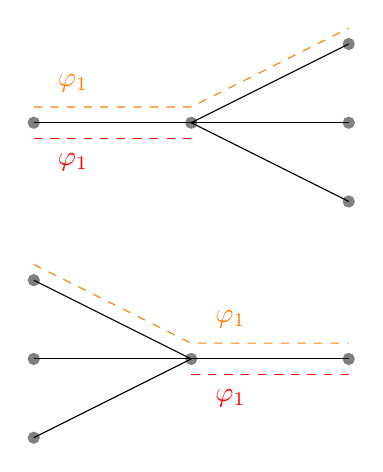
\begin{tikzpicture}
				%				[->,>=stealth',shorten >=1pt,auto,node distance=0,main node/.style={circle,draw}]
				\filldraw [gray] (0,2) circle (2pt)
				(2,2) circle (2pt)
				(4,3) circle (2pt)
				(4,2) circle (2pt)
				(4,1) circle (2pt);
				%
					\filldraw [gray] (4,-1) circle (2pt)
				(2,-1) circle (2pt)
				(0,0) circle (2pt)
				(0,-1) circle (2pt)
				(0,-2) circle (2pt);
				%
				\draw [black]  (0,2) -- (4,2);
				\draw [black]  (0,-1) -- (4,-1);
				%
				\draw [black] (2,2) -- (4,3);
				\draw [black] (2,2) -- (4,1);
				\draw [black] (0,0) -- (2,-1);
				\draw [black] (0,-2) -- (2,-1);
				%
				\draw [dashed, orange] (0,2.2) -> (2,2.2) -> (4,3.2);
				\draw [dashed, red] (0,1.8) -> (2,1.8);
				\draw [dashed, orange] (0,0.2) -> (2,-0.8) -> (4,-0.8);
				\draw [dashed, red] (2,-1.2) -> (4,-1.2);
				
	%		{\tiny
				\node [orange] at (0.5,2.5) {$\varphi_1$};	
				\node [red] at (0.5,1.5) {$\hsBt\varphi_1$};
			\node [orange] at (2.5,-0.5) {$\varphi_1$};	
				\node [red] at (2.5,-1.5) {$\hsEt\varphi_1$};
		%			\node (b0) at (4,-0.5) {$\rho'=\rho(0,i)\cdot \rho^{(j+1)]}$};	
		%			\node (a1) at (1.5,0.2) {$\rho(i)=$};
		%			\node (a2) at (2,0.2) {$\rho(j)$};
		%			\node (a3) at (1.65,0.5) {$Pattern(\rho,i)= Pattern(\rho,j)$};
		%			\node (a4) at (4.6,0.5) {$Pattern(\rho,k) =\{ p \in \Prop : \Ku,\rho^{k]} \models p\}$};
						
	%			}
				
			\end{tikzpicture}
\end{minipage}	
\hfill 	
\begin{minipage}{0.54\linewidth}
			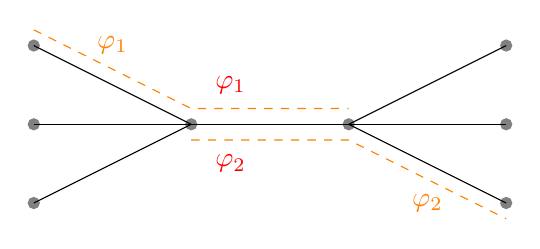
\begin{tikzpicture}
				%				[->,>=stealth',shorten >=1pt,auto,node distance=0,main node/.style={circle,draw}]
				%
					\filldraw [gray] (4,-1) circle (2pt)
				(2,-1) circle (2pt)
				(0,0) circle (2pt)
				(0,-1) circle (2pt)
				(0,-2) circle (2pt)
				(6,0) circle (2pt)
				(6,-1) circle (2pt)
				(6,-2) circle (2pt)	;
				%
				\draw [black]  (0,-1) -- (6,-1);
				%
				\draw [black] (4,-1) -- (6,0);
				\draw [black] (4,-1) -- (6,-2);
					\draw [black] (0,0) -- (2,-1);
				\draw [black] (0,-2) -- (2,-1);
				%
				\draw [dashed, orange] (0,0.2) -> (2,-0.8) -> (4,-0.8);
				\draw [dashed, orange] (2,-1.2) -> (4,-1.2) -> (6,-2.2);
				
	%		{\tiny
				\node [orange] at (1,0) {$\varphi_1$};	
				\node [red] at (2.5,-0.5) {$\hsAt\varphi_1$};
			\node [orange] at (5,-2) {$\varphi_2$};	
				\node [red] at (2.5,-1.5) {$\hsA \varphi_2$};
		%			\node (b0) at (4,-0.5) {$\rho'=\rho(0,i)\cdot \rho^{(j+1)]}$};	
		%			\node (a1) at (1.5,0.2) {$\rho(i)=$};
		%			\node (a2) at (2,0.2) {$\rho(j)$};
		%			\node (a3) at (1.65,0.5) {$Pattern(\rho,i)= Pattern(\rho,j)$};
		%			\node (a4) at (4.6,0.5) {$Pattern(\rho,k) =\{ p \in \Prop : \Ku,\rho^{k]} \models p\}$};
						
	%			}
				
			\end{tikzpicture}
\end{minipage}
%
    \caption{State-based semantic variant $\HS_\stat$: past and future are branching}
    \label{fig:ST}
\end{figure}